\documentclass[10pt]{ctexart}
\usepackage{graphicx, amsmath}
\usepackage{siunitx}
\usepackage[version=4]{mhchem}
\title{多晶X射线衍射的物相分析及其应用}
\author{张爱强\\指导教师: 王合英}
% The following parameters seem to provide a reasonable page setup.

\topmargin 0.0cm
\oddsidemargin 0.2cm
\textwidth 16cm 
\textheight 21cm
\footskip 1.0cm

\date{}
% set the section title format
\ctexset{
    section/format  += \raggedright
}
% set the abstract format
\newenvironment{sciabstract}{%
\begin{quote} \textbf{摘要: }}
{\end{quote}}
% set the bibliography format
\bibliographystyle{elsarticle-num}


\begin{document}
\maketitle
\begin{sciabstract}
    本实验使用X射线衍射测量多晶的衍射谱并利用Jade分析软件进行衍射谱标定。利用多晶X射线衍射仪对实验材料进行扫描,获得X射线的衍射谱。使用Jade
    对X射线衍射谱进行寻峰,匹配出对应的布拉格晶格结构,并利用物相数据库对X射线谱进行匹配,获得标定的物质信息。
    \par\textbf{关键词: } 多晶X射线衍射;Jade;布拉格晶格;物相数据库 .
\end{sciabstract}
\section{引言}
多晶X射线衍射分析是一种重要的物理化学实验方法。\texttt{物相分析}(根据晶体结构数据进行固态物质的物相组成分析,即物相定性分析及物相定量分析);测定晶
态物质的晶体结构参数以及与之有关的物理常数或物理量(如晶体的密度、热膨胀系数、金属材料中的宏观应力等);精确测量物质微观结构的微小变化(研究薄膜的结构与性能的关
系,催化剂的结构与催化性能的关系,研究亚微观晶粒的大小及其分布或晶粒中的缺陷等);材料结构分析。

本实验利用X射线衍射仪进行物相定性分析,并且使用数据库对未知材料进行标定。
\section{实验}
\subsection{实验仪器}
测角仪:常用的工作模式有$\theta/2\theta$和$\theta\theta$工作模式,本实验采用的是$\theta\theta$模式,即X射线仪旋转$\theta$,探测器旋转$\theta$。

Jade分析软件:X射线物相分析软件,可以对X射线衍射谱进行处理和分析,比如寻峰,确定衍射峰对应的Bragg晶格结构。同时可以和PDF数据库中的物品进行对比,查询标准卡。
\subsection{实验内容}
\begin{enumerate}
    \item 开启冷却水,开启X射线衍射仪,打开衍射仪控制软件,X射线衍射仪使用Cu靶,对应的波长为$\lambda=1.54059\times 10^{-10}m$
    \item 放入样品,调整扫描角度,用衍射仪获得衍射谱,保存为$element$.txt
    \item 将衍射谱导入Jade分析软件,调整寻峰使用的本底,峰的大小,寻峰,保存结果为$element$.pid;使用寻找到的峰位在数据库中查找,并比对标准卡片,保存结果为PDF.txt。
    \item 使用\ce{Si},\ce{NaCl}单晶,\ce{NaCl}多晶,\ce{Cu},\ce{Mo},\ce{W},石墨,金刚石粉,承载样品的基底,重复2,3步
    \item 关闭软件,关闭X射线衍射仪,10分钟后关闭冷却水
\end{enumerate}
\section{实验结果及讨论}
\subsection{\ce{Si}}
获得\ce{Si}衍射谱如图,对仪器的测量结果进行校验
\begin{figure}[htbp]
    \centering
    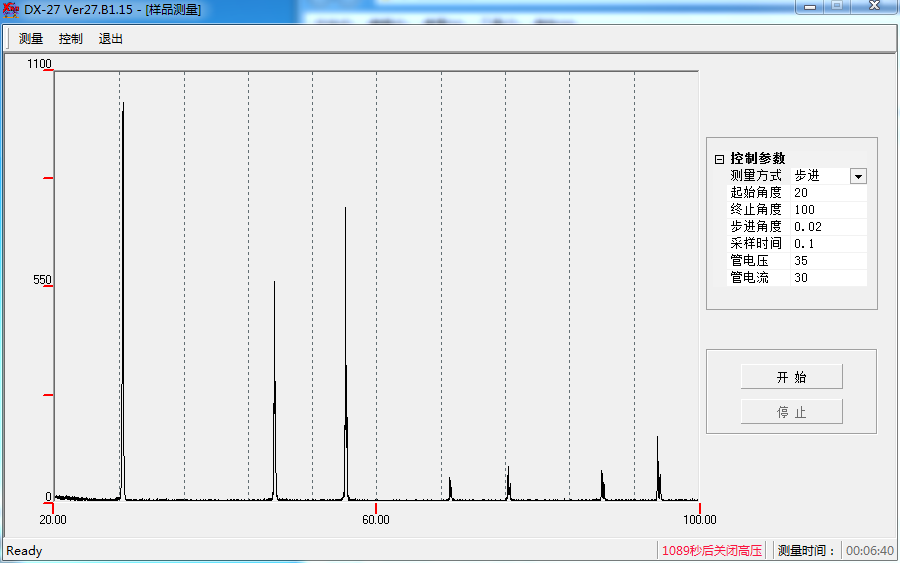
\includegraphics[width=0.7\textwidth]{data/Si/si.png}
    \caption{X射线谱仪测量能谱}
    \label{fig:SiXspec}
\end{figure}
\begin{figure}[htbp]
    \centering
    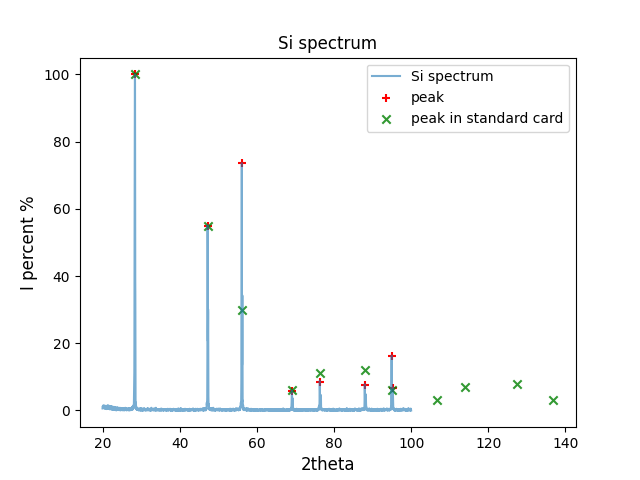
\includegraphics[width=0.7\textwidth]{data/Si/spectrum.png}
    \caption{Si分析软件寻峰及标准卡片}
    \label{fig:SiJadespec}
\end{figure}
利用Jade软件寻峰给出的结果与标准卡片对比,如图\ref{fig:SiJadespec},可以看出对于峰位角度衍射仪和标准卡片的结果完全一致。从寻峰给出的结果
可以得到对应的$\sin^2{\theta}$的值.

\begin{minipage}{0.45\textwidth}
{\small
\begin{tabular}{|c|c|c|c|}
    \textbf{Peak Index} & \textbf{$\sin^2{\theta}$}& \textbf{ratio}& \textbf{structure}\\
    \hline
    0  &  0.060167&3&(111)\\
1   & 0.160529&8&(220)\\
2  &  0.221077&11&(311)\\
3  &  0.321476&16&(222)\\
4  &  0.381742&19&\\
5  &  0.482402&&\\
6  &  0.543030&&\\
7  &  0.545516&&\\
\end{tabular}
\centering
Si的$\sin^2{\theta}$比值
\label{tab:SiPeakRatio}
}
\end{minipage}
\begin{minipage}{0.5\textwidth}
    可以从图\ref{fig:SiJadespec}看到由于扫描范围有限,所以图中绿色的点(标准卡片中的点在$120^\circ$之外仍然有存在的值)。从表\ref{tab:SiPeakRatio}可以
    看出\ce{Si}的晶体结构是面心立方结构,但是对应的晶面指数为$(200)(222)$并没有出现,可能是由于衍射峰强度不够强。

    利用衍射面指数$(111)$的角度$2d\sin{14.199^\circ}=\lambda$可以得到$d=3.14\times 10^{-10}m$,可以求出晶格常数
    \[a=\sqrt{h^2+k^2+l^2}d\]
    可以得到\SI{5.44}{\angstrom}
\end{minipage}
\subsection{基底}
因为放置样品的托盘基底也会产生影响,所以单独对基底进行X射线衍射测量得到图\ref{fig:base}
\begin{figure}[htbp]
    \centering
    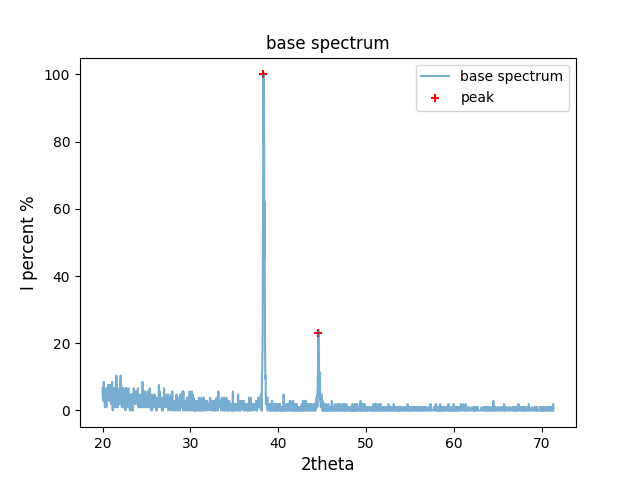
\includegraphics[width=0.7\textwidth]{data/base/spectrum.png}
    \caption{托盘基底的X衍射谱}
    \label{fig:base}
\end{figure}
其中对应的两个峰分别位于$2\theta=38.322 and 44.578$,因此测量其它样品时对应的这两个位置在样品衍射峰与这两个峰强度可比时,会出现在衍射图谱中。
\subsection{\ce{NaCl}}

分别对\ce{NaCl}单晶,\ce{NaCl}多晶进行测量获得衍射谱如图\ref{fig:NaCl}
\begin{figure}[htbp]
    \centering
    \begin{minipage}{0.45\textwidth}
        \centering
        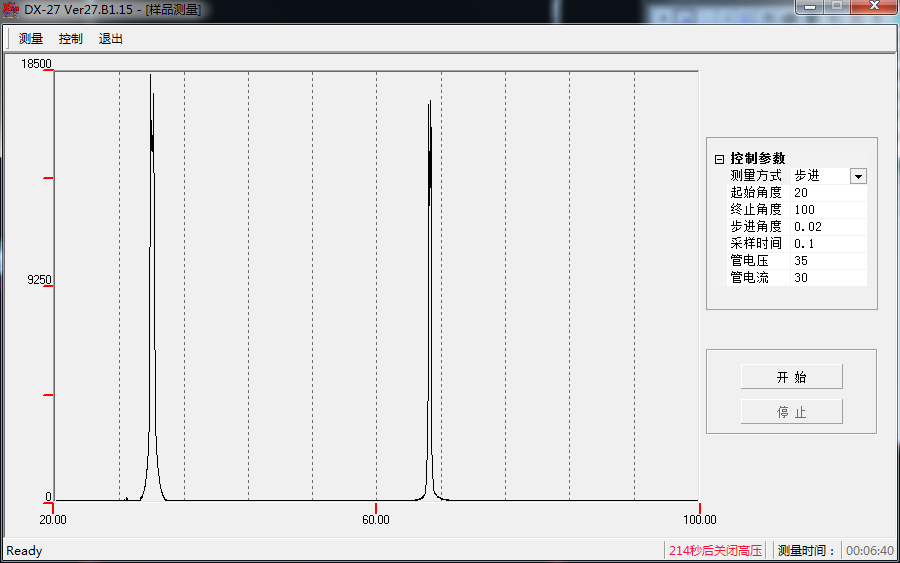
\includegraphics[width=\textwidth]{data/NaCl_s/nacl.png}
    \end{minipage}
    \qquad
    \begin{minipage}{0.45\textwidth}
        \centering
        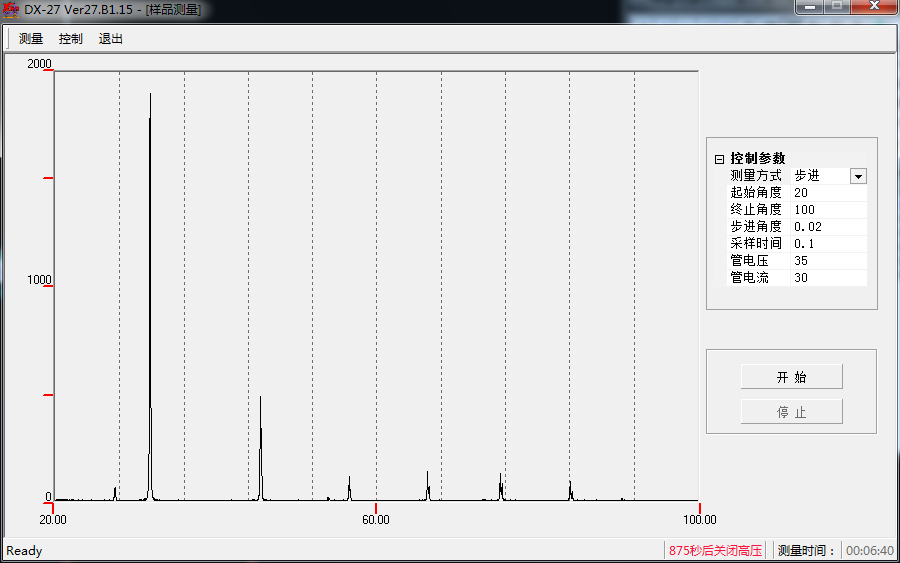
\includegraphics[width=\textwidth]{data/NaCl_m/nacl.png}
    \end{minipage}
    \caption{图a为NaCl单晶,图b为NaCl多晶}
    \label{fig:NaCl}
\end{figure}
利用Jade软件寻峰给出的结果与标准卡片对比,如图\ref{fig:NaClSJadespec}和图\ref{fig:NaClMJadespec},可以看出对于峰位角度衍射仪和标准卡片的结果完全一致。从寻峰给出的结果
可以得到对应的$\sin^2{\theta}$的值.
\begin{figure}
    \centering
    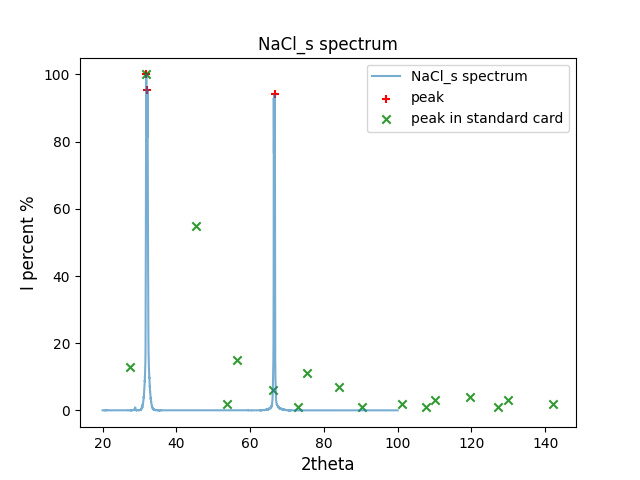
\includegraphics[width=0.7\textwidth]{data/NaCl_s/spectrum.png}
    \caption{\ce{NaCl}单晶的寻峰结果}
    \label{fig:NaClSJadespec}
\end{figure}
\begin{figure}
    \centering
    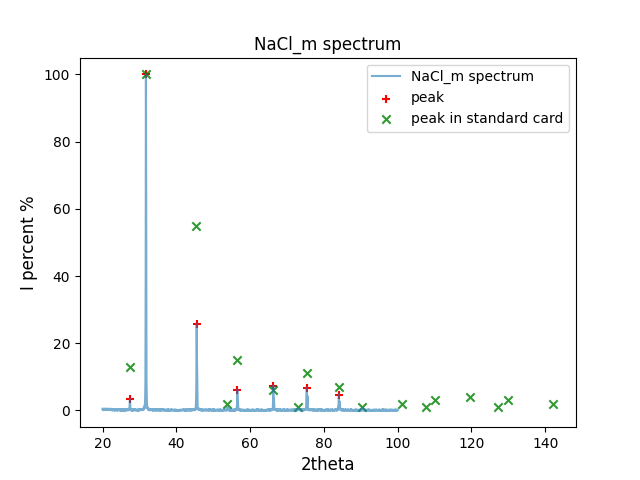
\includegraphics[width=0.7\textwidth]{data/NaCl_m/spectrum.png}
    \caption{\ce{NaCl}多晶的寻峰结果}
    \label{fig:NaClMJadespec}
\end{figure}
需要注意在给出的寻峰结果中有很多衍射峰并不存在,在表格\ref{tab:NaCl_sPeakRatio}中列出了衍射峰对应的面指数与$\sin^2{\theta}$的比值。

从\ce{NaCl}单晶的衍射峰角度比上可以看出是符合$1:4$关系,所以NaCl为简单立方或体心立方或者是面心立方结构。因为NaCl单晶的
取向在做X射线衍射时不多,所以很多衍射峰会被漏掉。这点可以通过使用\ce{NaCl}多晶进行X射线衍射来解决。

从\ce{NaCl}多晶的衍射峰角度比可以看出符合$3:4:8:12:16...$,所以基本可以排除简单立方和体心立方关系,认定NaCl晶格结构为面心立方结构,\textbf{其实仍然有一定可能性是简单立方}。而实际上NaCl是由两套
面心立方晶格构成的复式晶格,即\ce{Na}和\ce{Cl}分别形成一套Bragg晶格。\cite{gutiPhys}

另外从衍射峰强度之比,多晶NaCl的最强峰在$\sin^2{\theta}= 31.693^\circ$,可以wait to caculate.

\begin{minipage}{0.45\textwidth}
    {\small
    \begin{tabular}{|c|c|c|c|}
        \textbf{Peak Index} & \textbf{$\sin^2{\theta}$}& \textbf{ratio}& \textbf{structure}\\
        \hline
        0  &  0.075325&1&( 2 0 0)\\
    1  &  0.301746&4&( 4 0 0)\\
    \end{tabular}
    }
    \centering
    NaCl单晶的$\sin^2{\theta}$比值
    \label{tab:NaCl_sPeakRatio}
    
\end{minipage}
\begin{minipage}{0.45\textwidth}
    {\small
    \begin{tabular}{|c|c|c|c|}
        \textbf{Peak Index} & \textbf{$\sin^2{\theta}$}& \textbf{ratio}& \textbf{structure}\\
        \hline
        0  &  0.056245&3&( 111)\\
        1  &  0.075325&4&( 2 0 0)\\
        2  &  0.149670&8&( 220)\\
        3  &  0.224344&12&( 311)\\
        4  &  0.299002&16&( 222)\\
        5  &  0.373619&20&( 4 0 0)\\
        6  &  0.448248&24&(331)\\
    \end{tabular}
    }
    \centering
    NaCl多晶的$\sin^2{\theta}$比值
    \label{tab:NaCl_mPeakRatio}
\end{minipage}
\subsection{非金属}
\subsubsection{diamond}
获得衍射谱如图\ref{fig:diamond}
\begin{figure}
    \centering
    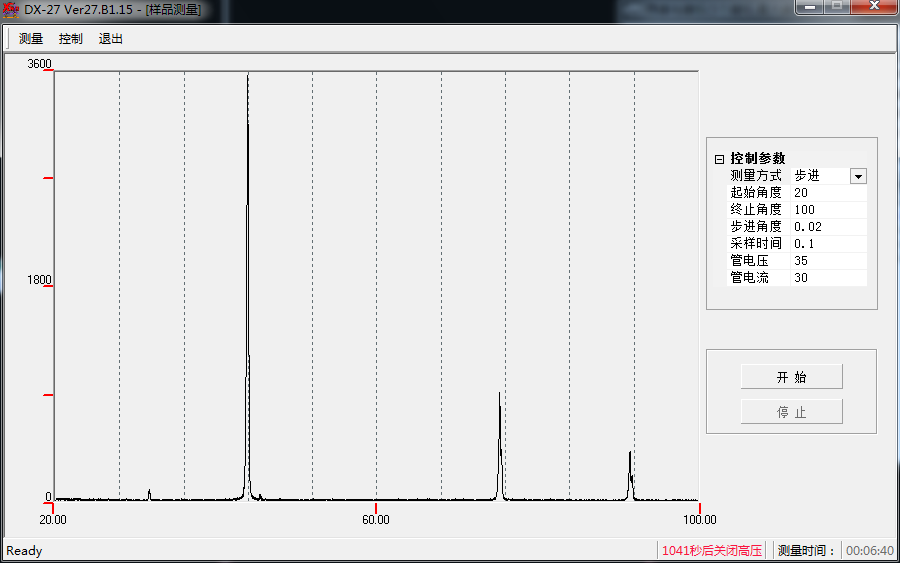
\includegraphics[width=0.7\textwidth]{data/diamond/diamond.png}
    \caption{金刚石的衍射谱}
    \label{fig:diamond}
\end{figure}
利用Jade软件寻峰给出的结果如图\ref{fig:diamond},和标准卡的结果正确吻合上。
\begin{figure}
    \centering
    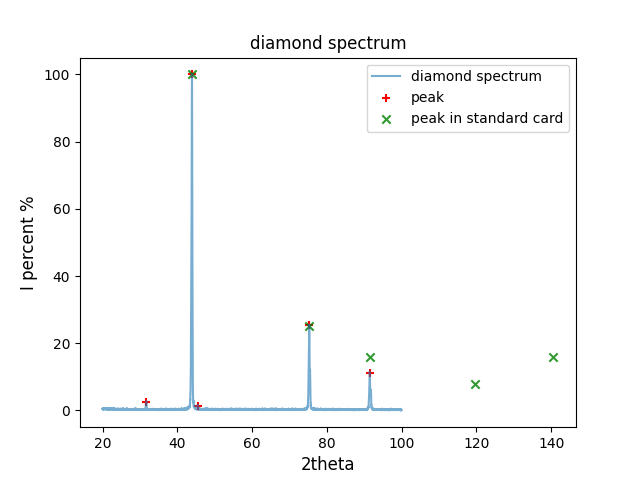
\includegraphics[width=0.7\textwidth]{data/diamond/spectrum.png}
    \caption{金刚石的寻峰结果}
    \label{fig:diamondJadespec}
\end{figure}
从表格\ref{tab:diamondPeakRatio}中可以发现金刚石的比值数列和面心立方和体心立方都不符合,\textbf{实际上第一个峰应该是其它杂质
引起的},比如第一个峰的位置的角度和\ce{NaCl}的第一个峰角度非常接近。而且实际上在第一个峰对应的2倍,在图\ref{fig:diamondJadespec}中是第三个
红色加号位置,应该是杂质的二级衍射。

所以综上讨论,排除掉第一个小峰,那么就和标准卡片给出的结果吻合,比值数列为$3:8:11$,确认结构为面心立方结构。\textbf{实际上金刚石是由两组面心立方晶格组成的复式晶格\cite{gutiPhys}}。
\begin{table}
    \begin{tabular}{|c|c|c|c|}
        \textbf{Peak Index} & \textbf{$\sin^2{\theta}$}& \textbf{ratio}& \textbf{structure}\\
        \hline
        0  &  0.074594&8&\\
    1   & 0.139839&15&\\
    2  &  0.372952&40&\\
    3  &  0.512905&55&\\
    \end{tabular}
    \centering
    金刚石的$\sin^2{\theta}$比值
    \label{tab:diamondPeakRatio}
\end{table}
\subsubsection{graphite}
\textbf{以下部分将不再给出X衍射仪给出的衍射谱截图,因为与寻峰结果中的图像重复。}

利用Jade软件寻峰给出的结果如图\ref{fig:graphite},可以看到仅有3个峰和标准卡片符合,对应的
三个峰的比值数列为$0.05268869:0.14374198:0.21035938=1:3:4$,所以可能是面心立方或者简单立方。

实际上石墨是层状结构,并没有明显的晶格结构。
\begin{figure}
    \centering
    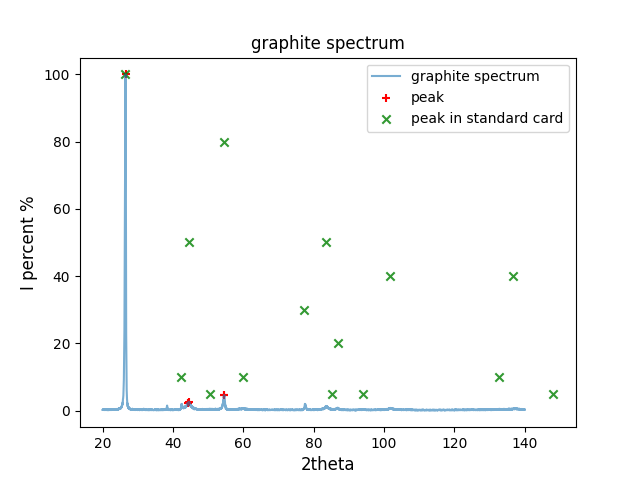
\includegraphics[width=0.7\textwidth]{data/graphite/spec.png}
    \caption{graphite的寻峰结果}
    \label{fig:graphite}
\end{figure}

\subsubsection{graphene}
利用Jade软件寻峰给出的结果如图\ref{fig:graphene},可以看到仅有3个峰和标准卡片符合,对应的
三个峰的比值数列为$0.052063:0.209230=1:4$
\begin{figure}
    \centering
    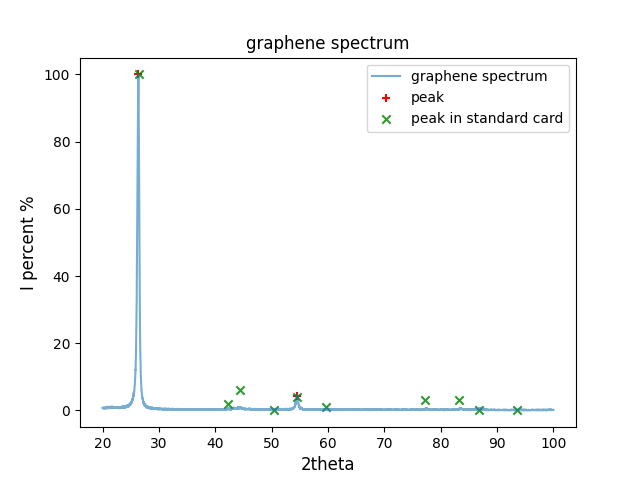
\includegraphics[width=0.7\textwidth]{data/graphene/spectrum.png}
    \caption{graphene的寻峰结果}
    \label{fig:graphene}
\end{figure}
\subsection{金属}
\subsubsection{金属\ce{Cu}}

利用Jade软件寻峰给出的结果如图\ref{fig:Cu}
\begin{figure}
    \centering
    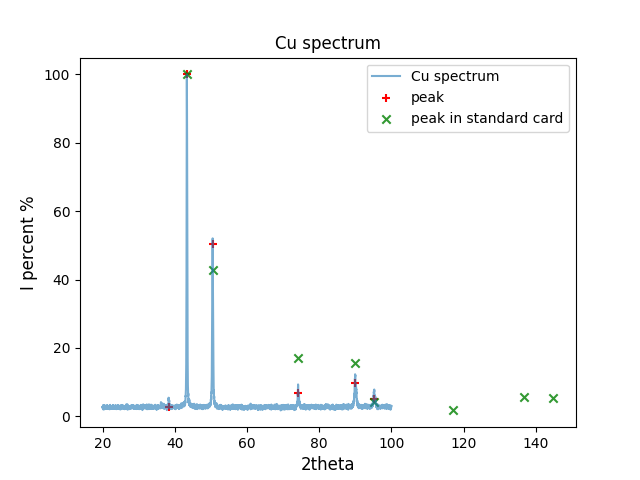
\includegraphics[width=0.7\textwidth]{data/Cu/spectrum.png}
    \caption{\ce{Cu}的寻峰结果}
    \label{fig:Cu}
\end{figure}
从表格\ref{tab:CuPeakRatio}中可以发现\ce{Cu}的第一个峰是\textbf{基底衍射产生的峰
引起的},第一个峰的位置的角度$2\theta=38.326^\circ$。

所以综上讨论,排除掉第一个小峰,那么就和标准卡片给出的结果吻合,比值数列为$3:4:8:11:12$,确认结构为面心立方结构。
\begin{table}
    \begin{tabular}{|c|c|c|c|}
        \textbf{Peak Index} & \textbf{$\sin^2{\theta}$}& \textbf{ratio}& \textbf{structure}\\
        \hline
0  &  0.107655&&\\
1  &  0.1364673&3&\\
2  &  0.181947&4&\\
3  &  0.363524&8&\\
4  &  0.499668&11&\\
5  &  0.545812&12&\\
    \end{tabular}
\centering
\caption{Cu的$\sin^2{\theta}$比值}
    \label{tab:CuPeakRatio}
\end{table}
\subsubsection{金属\ce{Mo}}
利用Jade软件寻峰给出的结果如图\ref{fig:Mo}
\begin{figure}
    \centering
    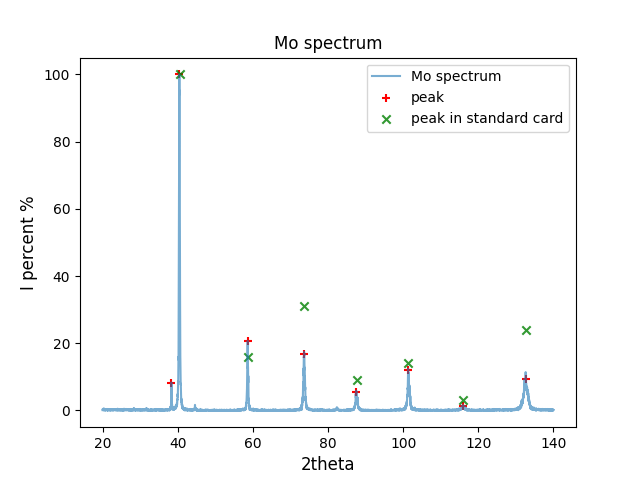
\includegraphics[width=0.7\textwidth]{data/Mo/spectrum.png}
    \caption{\ce{Mo}的寻峰结果}
    \label{fig:Mo}
\end{figure}
从表格\ref{tab:MoPeakRatio}中可以发现\ce{Mo}的第一个峰是\textbf{基底衍射产生的峰
引起的},第一个峰的位置的角度$2\theta=38.326^\circ$。而且在第二个加号对应的峰(并未在图中标出)恰好
和基底的另外一个衍射峰匹配。所以确认排除掉第一个衍射峰。

所以综上讨论,排除掉第一个小峰,那么就和标准卡片给出的结果吻合,比值数列为$1:2:3:4:5:6:7=2:4:6:8:10:12:14$,确认结构为体心立方结构。
\begin{table}
    \begin{tabular}{|c|c|c|c|}
        \textbf{Peak Index} & \textbf{$\sin^2{\theta}$}& \textbf{ratio}& \textbf{structure}\\
        \hline
0  &  0.107752&&\\
1  &  0.119463&1&\\
2  &  0.239629&2&\\
3  &  0.359164&3&\\
4  &  0.478182&4&\\
5  &  0.598307&5&\\
6  &  0.719311&6&\\
7  &  0.838425&7&\\
\end{tabular}
\centering
    \caption{Mo的$\sin^2{\theta}$比值}
    \label{tab:MoPeakRatio}
\end{table}
\subsection{混合物的定性物相分析}
\subsubsection{混合物1}
利用Jade软件寻峰给出的结果如图\ref{fig:hunhewu1}
\begin{figure}
    \centering
    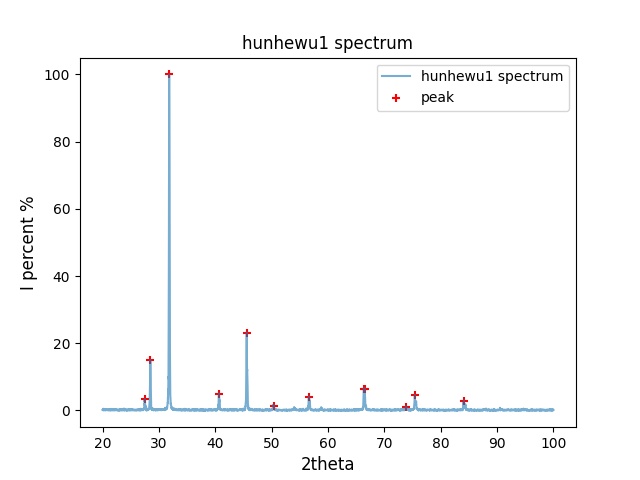
\includegraphics[width=0.7\textwidth]{data/hunhewu1/spectrum.png}
    \caption{混合物1的寻峰结果}
    \label{fig:hunhewu1}
\end{figure}
利用Jade软件进行匹配,如图\ref{fig:hunhewu1Match},获得混合物中的成分可能为\ce{NaCl}和\ce{KCl}。
\begin{figure}
    \centering
    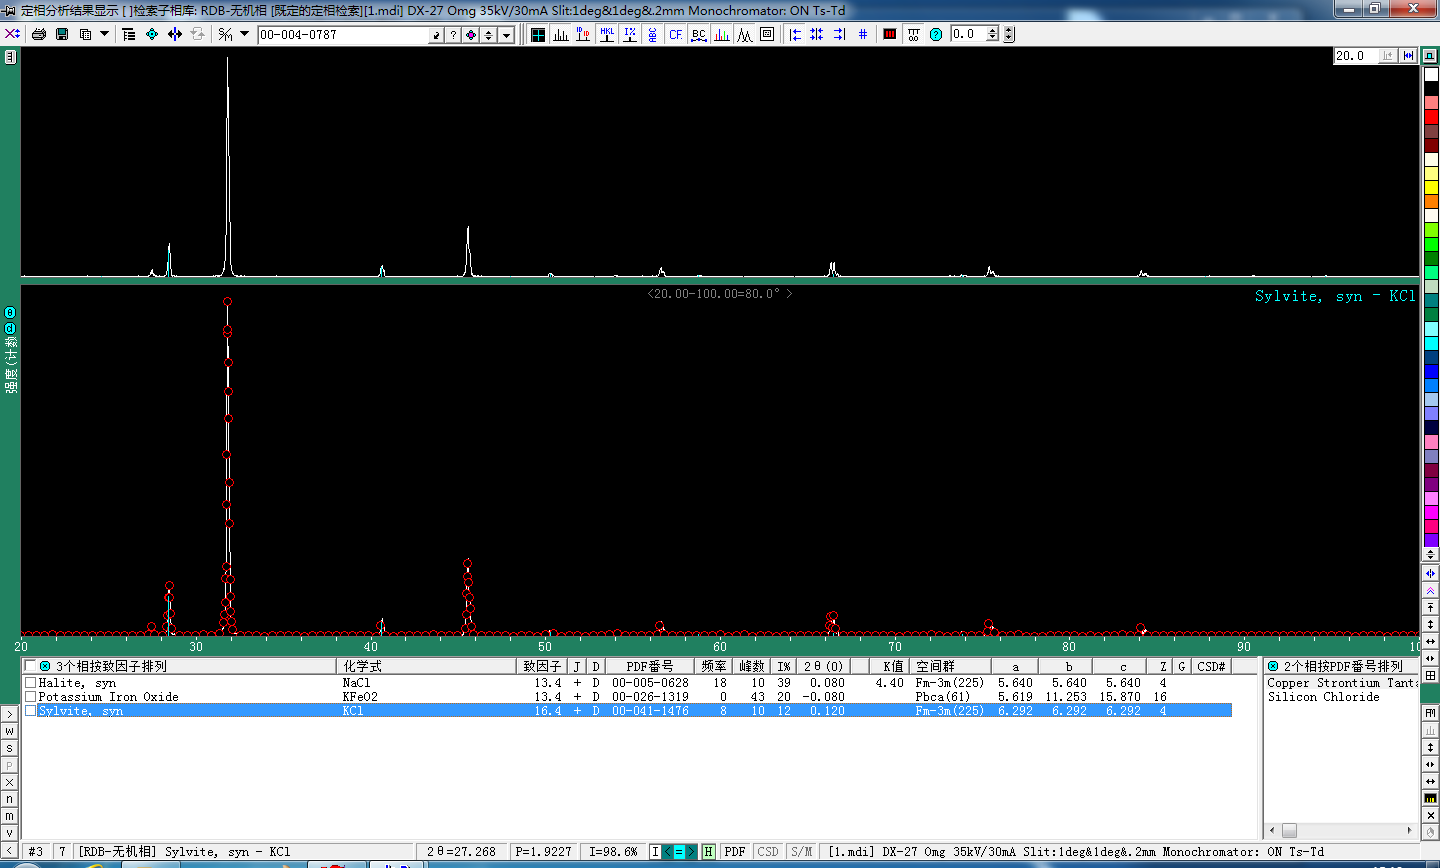
\includegraphics[width=0.7\textwidth]{data/hunhewu1/1.png}
    \caption{混合物1的匹配结果}
    \label{fig:hunhewu1Match}
\end{figure}
\subsubsection{混合物2}
利用Jade软件寻峰给出的结果如图\ref{fig:hunhewu2}
\begin{figure}
    \centering
    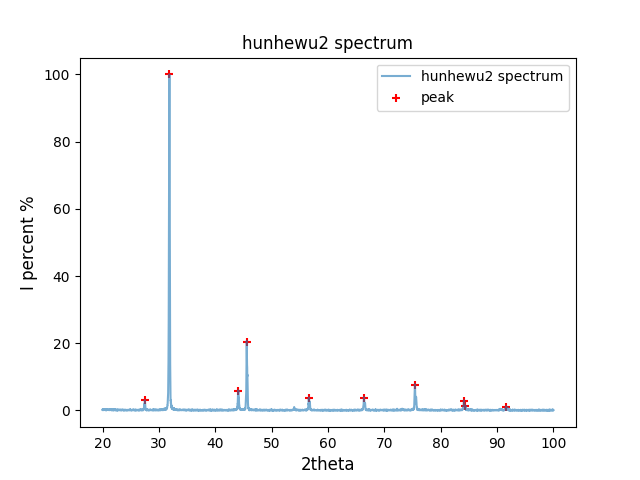
\includegraphics[width=0.7\textwidth]{data/hunhewu2/spectrum.png}
    \caption{混合物2的寻峰结果}
    \label{fig:hunhewu2}
\end{figure}
利用Jade软件进行匹配,如图\ref{fig:hunhewu2Match},获得混合物中的成分可能为\ce{NaCl}和\ce{Al}合金。
\begin{figure}
    \centering
    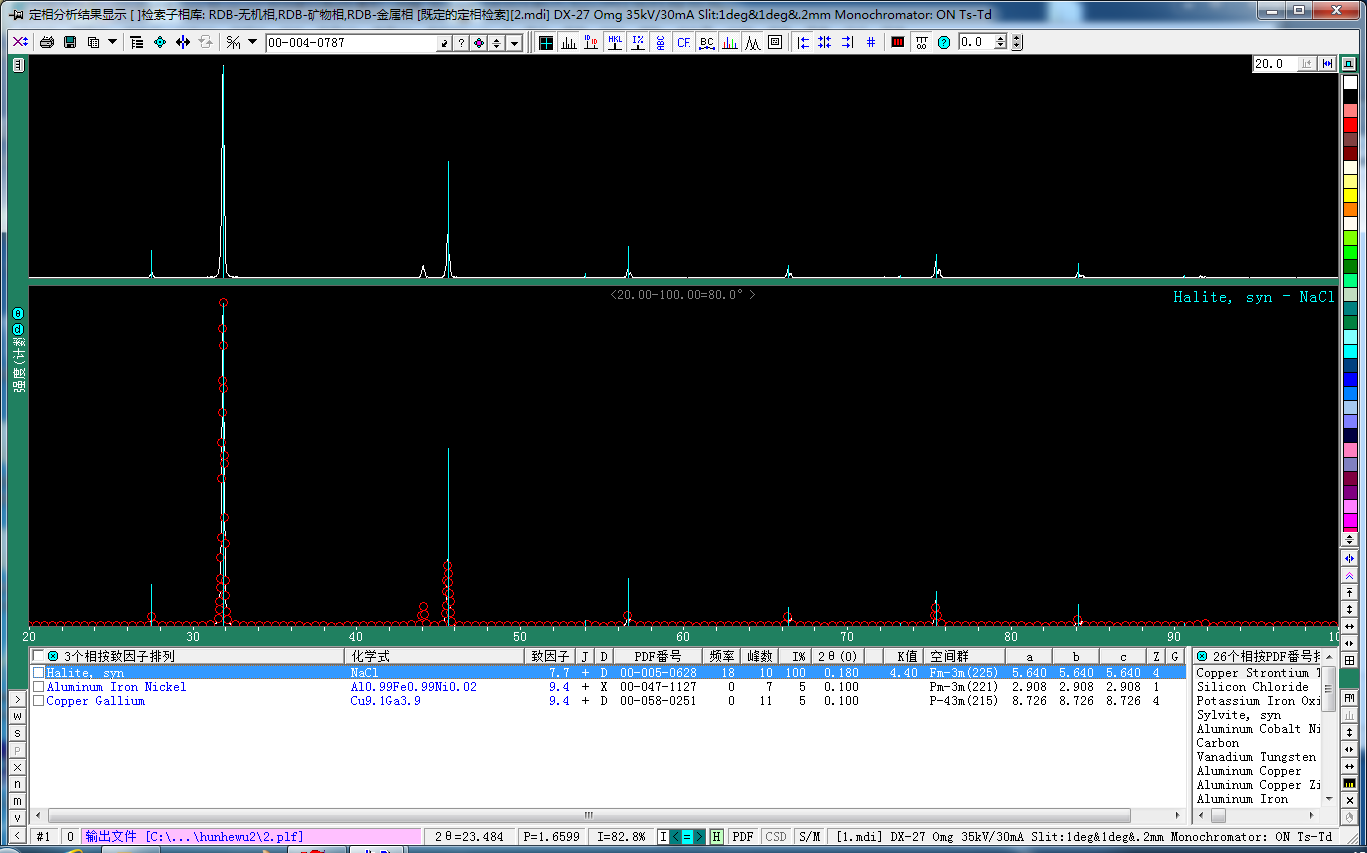
\includegraphics[width=0.7\textwidth]{data/hunhewu2/2.png}
    \caption{混合物2的匹配结果}
    \label{fig:hunhewu2Match}
\end{figure}
\section{结论}
本实验验证了衍射面指数对应衍射角的比例关系,利用衍射相对强度关系对混合物进行定标。
\subsection{思考}
\begin{enumerate}
    \item 实验中用的X单色光可以确定波长,通过滤波器或者多缝衍射(光栅)即可获得单色光。X射线衍射仪中使用石墨进行Bragg衍射获得单色光。
    \item $2d\sin{\theta}=n\lambda$的晶面对衍射峰有贡献
    \item 由于入射光角度原因,单晶可以发生衍射的晶面要少于多晶
    \item 物相分析通过比对衍射峰的结构来匹配晶体中的原子排列状态,无法获知原子的类别信息
    \item 实验测量的衍射峰比理论值偏大或偏小,可能是理论计算使用的入射的X射线波长与实际的X射线波长偏小或偏大
\end{enumerate}
\bibliography{report}
\end{document}